\documentclass[10pt, conference]{IEEEtran}
% \IEEEoverridecommandlockouts
% The preceding line is only needed to identify funding in the first footnote. If that is unneeded, please comment it out.
\usepackage{cite}
\usepackage{amsmath,amssymb,amsfonts}
\usepackage{algorithmic}
\usepackage{graphicx}
\usepackage{textcomp}
\usepackage{xcolor}
\usepackage{orcidlink}
\usepackage{acronym}
\def\BibTeX{{\rm B\kern-.05em{\sc i\kern-.025em b}\kern-.08em
    T\kern-.1667em\lower.7ex\hbox{E}\kern-.125emX}}


%---- PACKAGES
%\usepackage{todonotes}
\usepackage{amssymb}
\usepackage{hyperref}
\usepackage[plain]{fancyref}
\usepackage{ifdraft}
%\usepackage{subcaption}
\let\labelindent\relax
\usepackage[inline]{enumitem}
\usepackage{xcolor}
\usepackage{xspace}
\usepackage[final]{listings}
\usepackage{acronym}
\usepackage{url}
\usepackage{amsmath}
\usepackage{amssymb}
\usepackage{booktabs} % For formal tables
\usepackage{subfig}
\usepackage{balance}
\usepackage{dirtree}


\usepackage[ruled]{algorithm2e} % For algorithms
\renewcommand{\algorithmcfname}{ALGORITHM}
\newcommand{\subparagraph}{}
\usepackage[compact]{titlesec}
\titlespacing{\section}{0pt}{*0}{*0}
\titlespacing{\subsection}{0pt}{*0}{*0}
\titlespacing{\subsubsection}{0pt}{*0}{*0}

\usepackage{etoolbox}
\makeatletter
\patchcmd{\@makecaption}
  {\scshape}
  {}
  {}
  {}
\patchcmd{\@makecaption}
  {\\}
  {.\ }
  {}
  {}
\makeatother

%\let\refsection\relax
%\usepackage
%  [backend=bibtex,
%  style=ieee,
%   maxnames=5,
%   firstinits=true,
%   hyperref=true,
%   natbib=true,
%   url=false,
%   doi=false]{biblatex}



%
%----[ Biber ]----
%\addbibresource[datatype=bibtex]{local.bib}
%\addbibresource[datatype=bibtex]{bib/tools.bib}
%\addbibresource[datatype=bibtex]{bib/compsci.bib}
%\addbibresource[datatype=bibtex]{bib/learning.bib}
%\nocite{*}
%
%\newbibmacro{name:newformat}{%
%    \printnames{authors}
%%   \textbf{\namepartfamily}  % #1->\namepartfamily, #2->\namepartfamilyi
%%   \textbf{\namepartgiven}   % #3->\namepartgiven,  #4->\namepartgiveni
%%   [prefix: \namepartprefix] % #5->\namepartprefix, #6->\namepartprefixi
%%   [suffix: \namepartsuffix] % #7->\namepartsuffix, #8->\namepartsuffixi
%}
%
%\DeclareNameFormat{newformat}{%
%  \usebibmacro{name:newformat}{\textbf{#1}}{\textbf{#3}}{#5}{#7}%
%  \usebibmacro{name:andothers}%
%%  \nameparts{#1}% split the name data, will not be necessary in future versions
%%  \usebibmacro{name:newformat}%
%%  \usebibmacro{name:andothers}%
%}
%

%\AtEveryBibitem
%{
%   \clearlist{address}
%   \clearfield{date}
%   \clearfield{doi}
%   \clearfield{eprint}
%   \clearfield{isbn}
%   \clearfield{issn}
%   \clearfield{month}
%   \clearfield{note}
%%   \clearfield{pages}
%   \clearlist{location}
%%   \clearfield{series}
%   \clearfield{url}
%   \clearname{editor}
%   \ifentrytype{inproceedings}
%     {\clearfield{day}
%      \clearfield{month}
%      \clearfield{volume}}{}
%}
%
%\DeclareFieldFormat*{title}{\textsl{#1}\isdot}
%\DeclareFieldFormat*{journaltitle}{#1}
%\DeclareFieldFormat*{booktitle}{#1}
%
%\renewbibmacro{in:}{} % supress 'In: ' form
%
%\DeclareSourcemap
% {\maps[datatype=bibtex,overwrite]
%   {% Tag entries (through keywords)
%    \map
%      {\step[fieldsource=booktitle,
%       match=\regexp{[Pp]roceedings}, replace={Proc.}]}
%        \map
%      {\step[fieldsource=booktitle,
%       match=\regexp{[Ii]nternational\s+[Cc]onference}, replace={Intl. Conf.}]}
%    \map
%      {\step[fieldsource=journal,
%       match=\regexp{[Jj]ournal}, replace={Jour.}]}
%    \map
%      {\step[fieldsource=journal,
%       match=\regexp{[Tt]ransactions}, replace={Trans.}]}
%    \map
%      {\step[fieldsource=booktitle,
%       match=\regexp{[Pp]roceedings\s+of\s+the.+[Ee]uropean\s+[Cc]onference\s+in}, replace={European Conf. in}]}
%    \map
%      {\step[fieldsource=booktitle,
%       match=\regexp{In\s+[Pp]roceedings\s+of\s+the.+[Ss]ymposium\s+on}, replace={Symp. on}]}
%    \map
%      {\step[fieldsource=booktitle,
%       match=\regexp{[Pp]roceedings\s+of\s+the.+[Ii]nternational\s+[Cc]onference\s+on}, replace={Intl. Conf. on}]}
%    \map
%      {\step[fieldsource=booktitle,
%       match=\regexp{[Pp]roceedings\s+of\s+the.+[Ii]nternational\s+[Ww]orkshop\s+on}, replace={Intl. Workshop on}]}}}
%

%color
\definecolor{OliveGreen}{rgb}{0,0.6,0.3}

%References
%% Listings
\def\fref{\Fref} % treat all \frefs as \Frefs
\renewcommand{\lstlistingname}{Snippet}
\newcommand*{\fancyreflstlabelprefix}{lst}
\newcommand*{\Freflstname}{\lstlistingname}
\newcommand*{\freflstname}{\MakeLowercase{\lstlistingname}}
\Frefformat{vario}{\fancyreflstlabelprefix}%
  {\Freflstname\fancyrefdefaultspacing#1#3}
\frefformat{vario}{\fancyreflstlabelprefix}%
  {\freflstname\fancyrefdefaultspacing#1#3}
\Frefformat{plain}{\fancyreflstlabelprefix}%
  {\Freflstname\fancyrefdefaultspacing#1}
\frefformat{plain}{\fancyreflstlabelprefix}%
  {\freflstname\fancyrefdefaultspacing#1}

\renewcommand{\tablename}{Table}  
  
% ln delimiter
\newcommand*{\fancyreflnlabelprefix}{ln}
\newcommand*{\Freflnname}{Line}
\newcommand*{\freflnname}{\MakeLowercase{\Freflnname}}
\Frefformat{vario}{\fancyreflnlabelprefix}%
  {\Freflnname\fancyrefdefaultspacing#1#3}
\frefformat{vario}{\fancyreflnlabelprefix}%
  {\freflnname\fancyrefdefaultspacing#1#3}
\Frefformat{plain}{\fancyreflnlabelprefix}%
  {\Freflnname\fancyrefdefaultspacing#1}
\frefformat{plain}{\fancyreflnlabelprefix}%
  {\freflnname\fancyrefdefaultspacing#1}    


%JavaScript definition
\lstdefinelanguage{JavaScript}{
keywords={typeof, new, true, false, catch, function, return, null, catch, switch, var, if, in, for, while, do, else, case, break, throw, this, instanceof},
keywordstyle=\color{purple}\bfseries,
ndkeywords={},
ndkeywordstyle=\color{blue}\bfseries,
identifierstyle=\color{black},
sensitive=false,
comment=[l]{//},
morecomment=[s]{/*}{*/},
commentstyle=\color{OliveGreen}\ttfamily,
stringstyle=\color{OliveGreen}\ttfamily,
morestring=[b]',
morestring=[b]"
}
\usepackage{color}
\definecolor{gray97}{gray}{.97}
\definecolor{gray90}{gray}{.90}
\definecolor{gray75}{gray}{.75}
\definecolor{gray45}{gray}{.45}
\definecolor{codegreen}{rgb}{0,0.6,0}
\definecolor{codered}{rgb}{0.6,0,0}
\definecolor{codegray}{rgb}{0.5,0.5,0.5}
\definecolor{codepurple}{rgb}{0.58,0,0.82}
\lstset{ frame=single,
	framerule=0.2pt,
	framextopmargin=3pt,
	framexbottommargin=3pt,
	framexleftmargin=0.4cm,
	framesep=0.5pt,
	rulesep=0.5pt,
	backgroundcolor=\color{gray97},
	rulesepcolor=\color{black},
	xleftmargin=0.7cm,
	%
	stringstyle=\ttfamily,
	showstringspaces = false,
	basicstyle=\fontsize{6pt}{7pt}\ttfamily,
	keywordstyle=\color{magenta}\bfseries,
	numberstyle=\tiny\color{codegray},
	stringstyle=\color{codepurple},
	commentstyle=\color{codegreen},
	%
	numbers=left,
	numbersep=15pt,
	numberstyle=\tiny,
	numberfirstline = false,
	breaklines=true,
	escapeinside={(*@}{@*)},
	literate={~} {$\sim$}{1}
}

\lstdefinestyle{floating}{%
  frame=none,
  float=htb,
  captionpos=b
}

% context traits listings
\lstdefinestyle{ctxtraits}
 {language=JavaScript,
  frame=lines,
  showstringspaces=false,
  keywordstyle=\tt\bf,
  tabsize=3,
  style=floating,
  morekeywords={Trait, cop, Context, activate, deactivate, adapt, addObjectPolicy, manager}
}

%context traits environment    
\lstnewenvironment{ctxtraits}[1][]
 {\lstset{style=ctxtraits,#1}}{}  


 % Context Traits in line source code
\newcommand{\scode}[1]{\textrm{\texttt{#1}}}
\def\scode{\lstinline[style=ctxtraits]}

%----[ Commands ]---
%Latins
\newcommand{\eg}{\emph{e.g.,}\xspace}
\newcommand{\ie}{\emph{i.e.,}\xspace}
\newcommand{\etal}{\emph{et al.}\xspace}
\newcommand{\aka}{\emph{a.k.a.,}\xspace}
\newcommand{\cf}{\emph{cf.}\xspace}
\newcommand{\mref}{\textcolor{red}{[REF]}\xspace}
\newcommand{\secref}[1]{Section~\ref{#1}\xspace}
\newcommand{\figref}[1]{Fig.~\ref{#1}\xspace}
\newcommand{\listref}[1]{Listing~\ref{#1}\xspace}
\newcommand{\tabref}[1]{Table~\ref{#1}\xspace}

\newcommand{\itdroid}{\textsc{itDroid}\xspace}
\newcommand{\numapps}{\textcolor{red}{80}\xspace}


\newcommand{\ctx}[1]{\texttt{\textsc{#1}}}


%comments
% xcolor
\definecolor{author}{rgb}{.5, .5, .5}
\definecolor{comment}{rgb}{.1, .0, .9}
\definecolor{note}{rgb}{.9, .4, .0}
\definecolor{idea}{rgb}{.1, .7, .0}
\definecolor{missing}{rgb}{.9, .1, .0}
\definecolor{deleteme}{rgb}{.9, .1, .0}

\newcommand{\MARIO}[2][comment]{\authorcomment[#1]{MLV}{#2}}
\newcommand{\CAMILO}[2][comment]{\authorcomment[#1]{CEV}{#2}}
\newcommand{\ALEJO}[2][comment]{\authorcomment[#1]{AMR}{#2}}
\newcommand{\ANA}[2][comment]{\authorcomment[#1]{AMH}{#2}}
\newcommand{\MICHAEL}[2][comment]{\authorcomment[#1]{MOR}{#2}}
\newcommand{\LAURA}[2][comment]{\authorcomment[#1]{LBJ}{#2}}

\newcommand{\authorcomment}[3][comment]
  {\noindent
      \fbox{\footnotesize\textcolor{author}{\textsc{#2}}}
      \textcolor{#1}{\textsl{#3}}{}}




% !TEX root = main.tex

\acrodef{APK}{Android Application Package}
\acrodef{AI}{Artificial Intelligence}
\acrodef{WCAG}{Web Content Accessibility Guidelines}
\acrodef{UI}{User Interface}
\acrodef{AOM}{Accessibility Object Model}
% \acrodef{a11y}{Accessibility}
\begin{document}

\title{Autonomous Agents for Accessibility: Simulating Visual Impairments in Web Interfaces}

% \author{
%     \IEEEauthorblockN{
%         Juan Diego Yepes-Parra \orcidlink{0009-0007-0672-1473}, 
%         Camilo Escobar-Velásquez \orcidlink{0000-0001-8414-9301}
%     }
%     \IEEEauthorblockA{
%         \textit{Universidad de los Andes, Colombia} \\
%         \{j.yepes, ca.escobar2434\}@uniandes.edu.co
%     }
% }

\maketitle

\begin{abstract}
Static code analysis cannot detect real-time interaction issues faced by users with disabilities. We propose a multimodal \ac{AI} agent framework that simulates interactions of users with visual impairments without code access. 
The agent would closely simulate the experience of these users by interacting with web interfaces using the same modalities available to them, primarily keyboard navigation and screen readers. The agent perceives the interface through perceptual filters that mimic conditions including glaucoma and myopia, and handles both the altered visual input and audio output from screen readers. 
This approach aims to replicate the real-world constraints and strategies of users with disabilities, enabling more realistic evaluation, with the objective of identifying, locating and repairing web accessibility issues. 
We suggest a framework to evaluate how such filters affect user behavior, task success, and \ac{UI} usability. Our approach aims to uncover visual accessibility flaws that become apparent under impaired perception. 
\end{abstract}

\begin{IEEEkeywords}
Web Accessibility; Autonomous Artificial Intelligence Agents; Automated Testing
\end{IEEEkeywords}


% !TEX root = main.tex

\section{Introduction}

Web \ac{a11y} is central to inclusive software design, yet existing evaluation methods predominantly focus on code conformance, as illustrated by \ac{WCAG} rule checks, often overlooking how individuals with disabilities actually navigate and perceive interfaces in practice~\cite{ara2024inclusive}. Although these tools are useful for guidance and a first approach, they can be unable to thoroughly assess how these impairments affect real-time usability, task completion, or perception of interface elements. While often ignoring behavioral context; they do not simulate navigation, focus order, or sequential interaction flows that can significantly impact \ac{a11y}. Individuals with disabilities have diverse needs and experiences, many of which may not be fully addressed by level-A \ac{WCAG} guidelines alone.

Although the access to information is a human right, the urgency of dynamic and human-centered \ac{a11y} evaluation is also supported by data. Approximately 2.2 billion people globally have some sort of visual impairment, including both near and distant vision issues \cite{who2023vision}. In Colombia, among the estimated 2.65 million people living with a disability by the DANE, approximately 57\% report that vision-related activities present the greatest challenges\cite{DANE2022}. In bigger countries like the USA, the CDC reports that, about 5.5\% of adults (nearly 19 million people) have blindness or serious difficulty seeing\cite{cdc2025disabilities}. Furthermore, screen reader users find that the most problematic items to interact with in a webpage are CAPTCHA, interactive elements, ambiguous links or buttons, unexpected screen changes, lack of keyboard support, among others\cite{webaimsurvey2025}. Even more tellingly, these users extract information from data visualizations 61\% less accurately and take 211\% more time compared to sighted users \cite{wobbrock2021assets}.

We explore the possibility of approaching \ac{a11y} testing using autonomous \ac{AI} agents capable of interacting with websites while being exposed to simulated visual impairments. These agents are prompted with specific user tasks (e.g., locating a button, submitting a form) and attempt to complete them. The agents can also integrate outputs from assistive technologies, for example, capturing a screen reader's textual narration. 

This multi-modal input allows the agent to simulate how a user with various levels of visual impairment (glaucoma, cataracts, myopia or low vision, among others) interacts with content, opening the door for dynamic automated testing other existing tools might be unable to uncover. For instance, detecting unuseful alt text, mislabeled controls or mismatches between rendered content and screen reader output. 

This paper outlines our motivation, proposed approach, poses future evaluation research questions, and discusses implementation considerations for such a system.

% !TEX root = main.tex

\section{Related Work}
\subsection{Web a11y compliance}

Conventional web \ac{a11y} assessments primarily rely on static checkers that verify compliance with \ac{WCAG} criteria by inspecting HTML and CSS structures. Tools such as WAVE by WebAIM\cite{webaim_wave_2025} and IBM's NPM accessibility-checker\cite{ibm_accessibility_checker_2025} exemplify this approach. However, several studies have revealed significant limitations in these tools, noting they often lack semantic awareness and fail to consider user perspectives, leading to incomplete or misleading results \cite{ara2024inclusive}. 

For instance, Todorov et al. evaluated Bulgarian museum websites uncovered widespread \ac{a11y} failures despite technical correctness \cite{todorov2022accessibility}. Similarly, Inal et al. conducted a study of Norwegian municipal websites and found that although legislation mandated \ac{WCAG} compliance, issues such as low-quality alternative text persisted.
Chiou et al. further observed that many common web \ac{a11y} issues arise in responsive sites during resizing, highlighting the importance of evaluating \ac{a11y} across different device viewports\cite{chiou2024automatically}.

Complimentarily, \ac{WCAG} conformance varies by level, from A (lower) to AAA (higher), meaning that a website labeled as “compliant” may still fall short of more stringent and specific \ac{a11y} standards. These findings underscore the need for real-time evaluations that reflect how visually impaired users interact with web interfaces. 
While automated tools are useful for early feedback, they are unable to identify all critical \ac{a11y}, functionality, and usability issues affecting this population \cite{todorov2022accessibility}.

\subsection{Automated a11y Testing}

Recent studies introduce hybrid frameworks that combine guidelines with heuristic, automated, or AI-driven methods to improve a11y evaluation. Watanabe et al.~\cite{watanabe2024accessibility} show that machine learning can detect ARIA landmarks in web apps, revealing how classifiers may infer structure when key \ac{a11y} tags are missing. Similarly, models have been used to identify and remediate \ac{a11y} issues, helping sites align with accessibility standards. Some approaches analyze source code to suggest fixes~\cite{ramineni2024leveraging, kuszczynski2023comparative}, while others operate on rendered pages using prompt-based methods~\cite{he2025enhancing}. Mehralian et al.~\cite{mehralian2025automated} propose a rule-based system for testing dynamic content in Android apps, and Tafreshipour et al.~\cite{tafreshipour2024ma11y} show that mutation testing can uncover additional errors by exploring app states and applying accessibility rules. These efforts reflect growing recognition of the limits of static, rule-based tools, while still relying on source code analysis, not simulating user behavior.


\subsection{Autonomous AI agents}

The use of autonomous \ac{AI} agents to simulate user interaction with web interfaces has also been explored. Lu et al. \cite{lu2025uxagent} introduce UXAgent; a notable system that uses LLM agents to mimic thousands of diverse user personas in web usability studies. The agents interact with live websites via browser automation, providing qualitative and quantitative feedback that supports iterative UX design. 

Complementing this, a GitHub Copilot extension that proactively embeds \ac{a11y} guidance into the coding workflow was unveiled by Mowar et al. \cite{mowar2025codea11y}. Their study shows how \ac{AI} assistants can suggest accessible \ac{UI} code, highlight missing attributes, and prompt manual verification during development.

While not strictly agent-based, Zhong et al. \cite{zhong2025screenaudit} leveraged large language models to identify discrepancies between screen reader outputs, providing a novel approach to detecting accessibility errors.

Another recent advancement in this area is AXNav by Taeb et al. \cite{taeb2024axnav}, a system that interprets mobile \ac{a11y} test instructions written in natural language and executes them on remote cloud devices using an LLM-based multiagent planner. This approach demonstrates how LLM-driven agents can automate complex evaluations and provide actionable, context-rich feedback for developers.

Multimodal agents that adaptively present content based on user needs, transforming visual content into speech or simplified visuals for users with auditory or visual processing disorders were also proposed by Rajagopal et al. \cite{rajagopal2023design}. While not focused on web testing, their work shows how agents can model disability-specific interactions across modalities.


% !TEX root = main.tex

\section{Motivation}

The widespread adoption of the web has emphasized the importance of ensuring that online content is accessible to everyone, including individuals with various disabilities\cite{abu2023web}. Despite this, less than 4\% of the top one million websites are fully accessible. Over 96\% contain detectable \ac{WCAG} failures, with an average of 51 errors per page \cite{webaimmillion2025}. Common issues include missing alt text (present on 56\% of home pages), low contrast, and poor form labeling \cite{audioeye2024}.

%// Meanwhile, the legal landscape is becoming stricter. The European Accessibility Act mandates compliance by June 28, 2025 for both public and private digital services in the EU, affecting more than 87 million EU residents with disabilities \cite{audioeyeEAA2025, accessibleEU2025}. 
% no se si poner este parrafo

On the other hand, rigorous testing is integral to ensuring reliability of web applications. For example, usability testing that involves having real users interacting with a live web application, allows for the identification of issues in action, enables for iterative feedback and a more realistic assessment of how they might experience the interface. Effective testing improves satisfaction, avoids rework, and ensures genuinely inclusive design \cite{accessdesign2025}.

Although \ac{WCAG} articulate extensive criteria for inclusive design \cite{w3c_WCAG22}, existing tools focus more on compliance than on realistic user behavior. Developers and UX practitioners often lack practical mechanisms to validate these guidelines in realistic usage scenarios. For instance, some of the significant challenges found in testing are little room for iteration, lack of extensive and appropiate user feedback, and limitations to empathy-based research methods\cite{lu2025uxagent}.

%? parrafo del research gap que encontramos
Finally, while recent advances have demonstrated the potential of autonomous agents for usability testing\cite{lu2025uxagent} and mobile accessibility feature testing\cite{taeb2024axnav}, to our knowledge, no one has applied them for web accessibility evaluations yet. Bridging this gap offers the opportunity to deliver scalable, repeatable, and realistic assessments of how users with disabilities interact with web interfaces. Our hope is that we can significantly enhance the detection and remediation of accessibility issues, making the evaluation process more efficient and comprehensive.

\section{Automated Testing}

Dynamic testing can help developers and stakeholders verify and validate that running software is working as expected. In this case, automated testing is the enabler for faster, more reliable and overall optimized testing. Automated testing leveraged by machine learning and \ac{AI} are increasingly becoming more popular and sophisticated, therefore using them in this scenario is a big step forward for ensuring accessibility. %*aqui seria bueno poner una referencia de TSDL

Intelligent agents can interact with web content without access to the underlying code, relying instead on the same content the final user is interacting with\cite{lanham2025ai, wang2024survey, lu2025uxagent}. They can also be adapted based on feedback, and can process rich multimodal inputs, such as screenshots and screen reader text, enabling them to reason about both the visual layout and the spoken feedback of the user interface simultaneously. They are also able to use different interaction techniques, like keyboard only, mouse only, etc. 

Finally, LLM agents excel at open-ended reasoning and can provide qualitative insights, alongside quantitative logs. However, they require careful prompting and can be slower or less predictable.


\section{Objectives}

First, we aim to explore the use of perceptual filters and multimodal inputs, such as applying blur to simulate different impairments; while also using screen reader outputs, to approximate the experience of real world users. 

Additionally, we will analyze whether certain \ac{UI} elements become inaccessible or difficult to perceive under these simulated conditions, and investigate if common layout structures or design patterns can fail in these situations. Through this approach, we seek to identify not only the direct effects of visual filters on usability, but also the broader structural and behavioral implications for accessible web design.

\section{System design}
\subsection{Visual Filtering}

Simulating visual impairments through perceptual filters allows us to approximate the experiences of users with conditions such as glaucoma and myopia. These filters alter the rendered webpage in ways that reflect known physiological effects, such as peripheral vision loss, blur, or reduced contrast sensitivity.

\begin{figure}
    \centering
    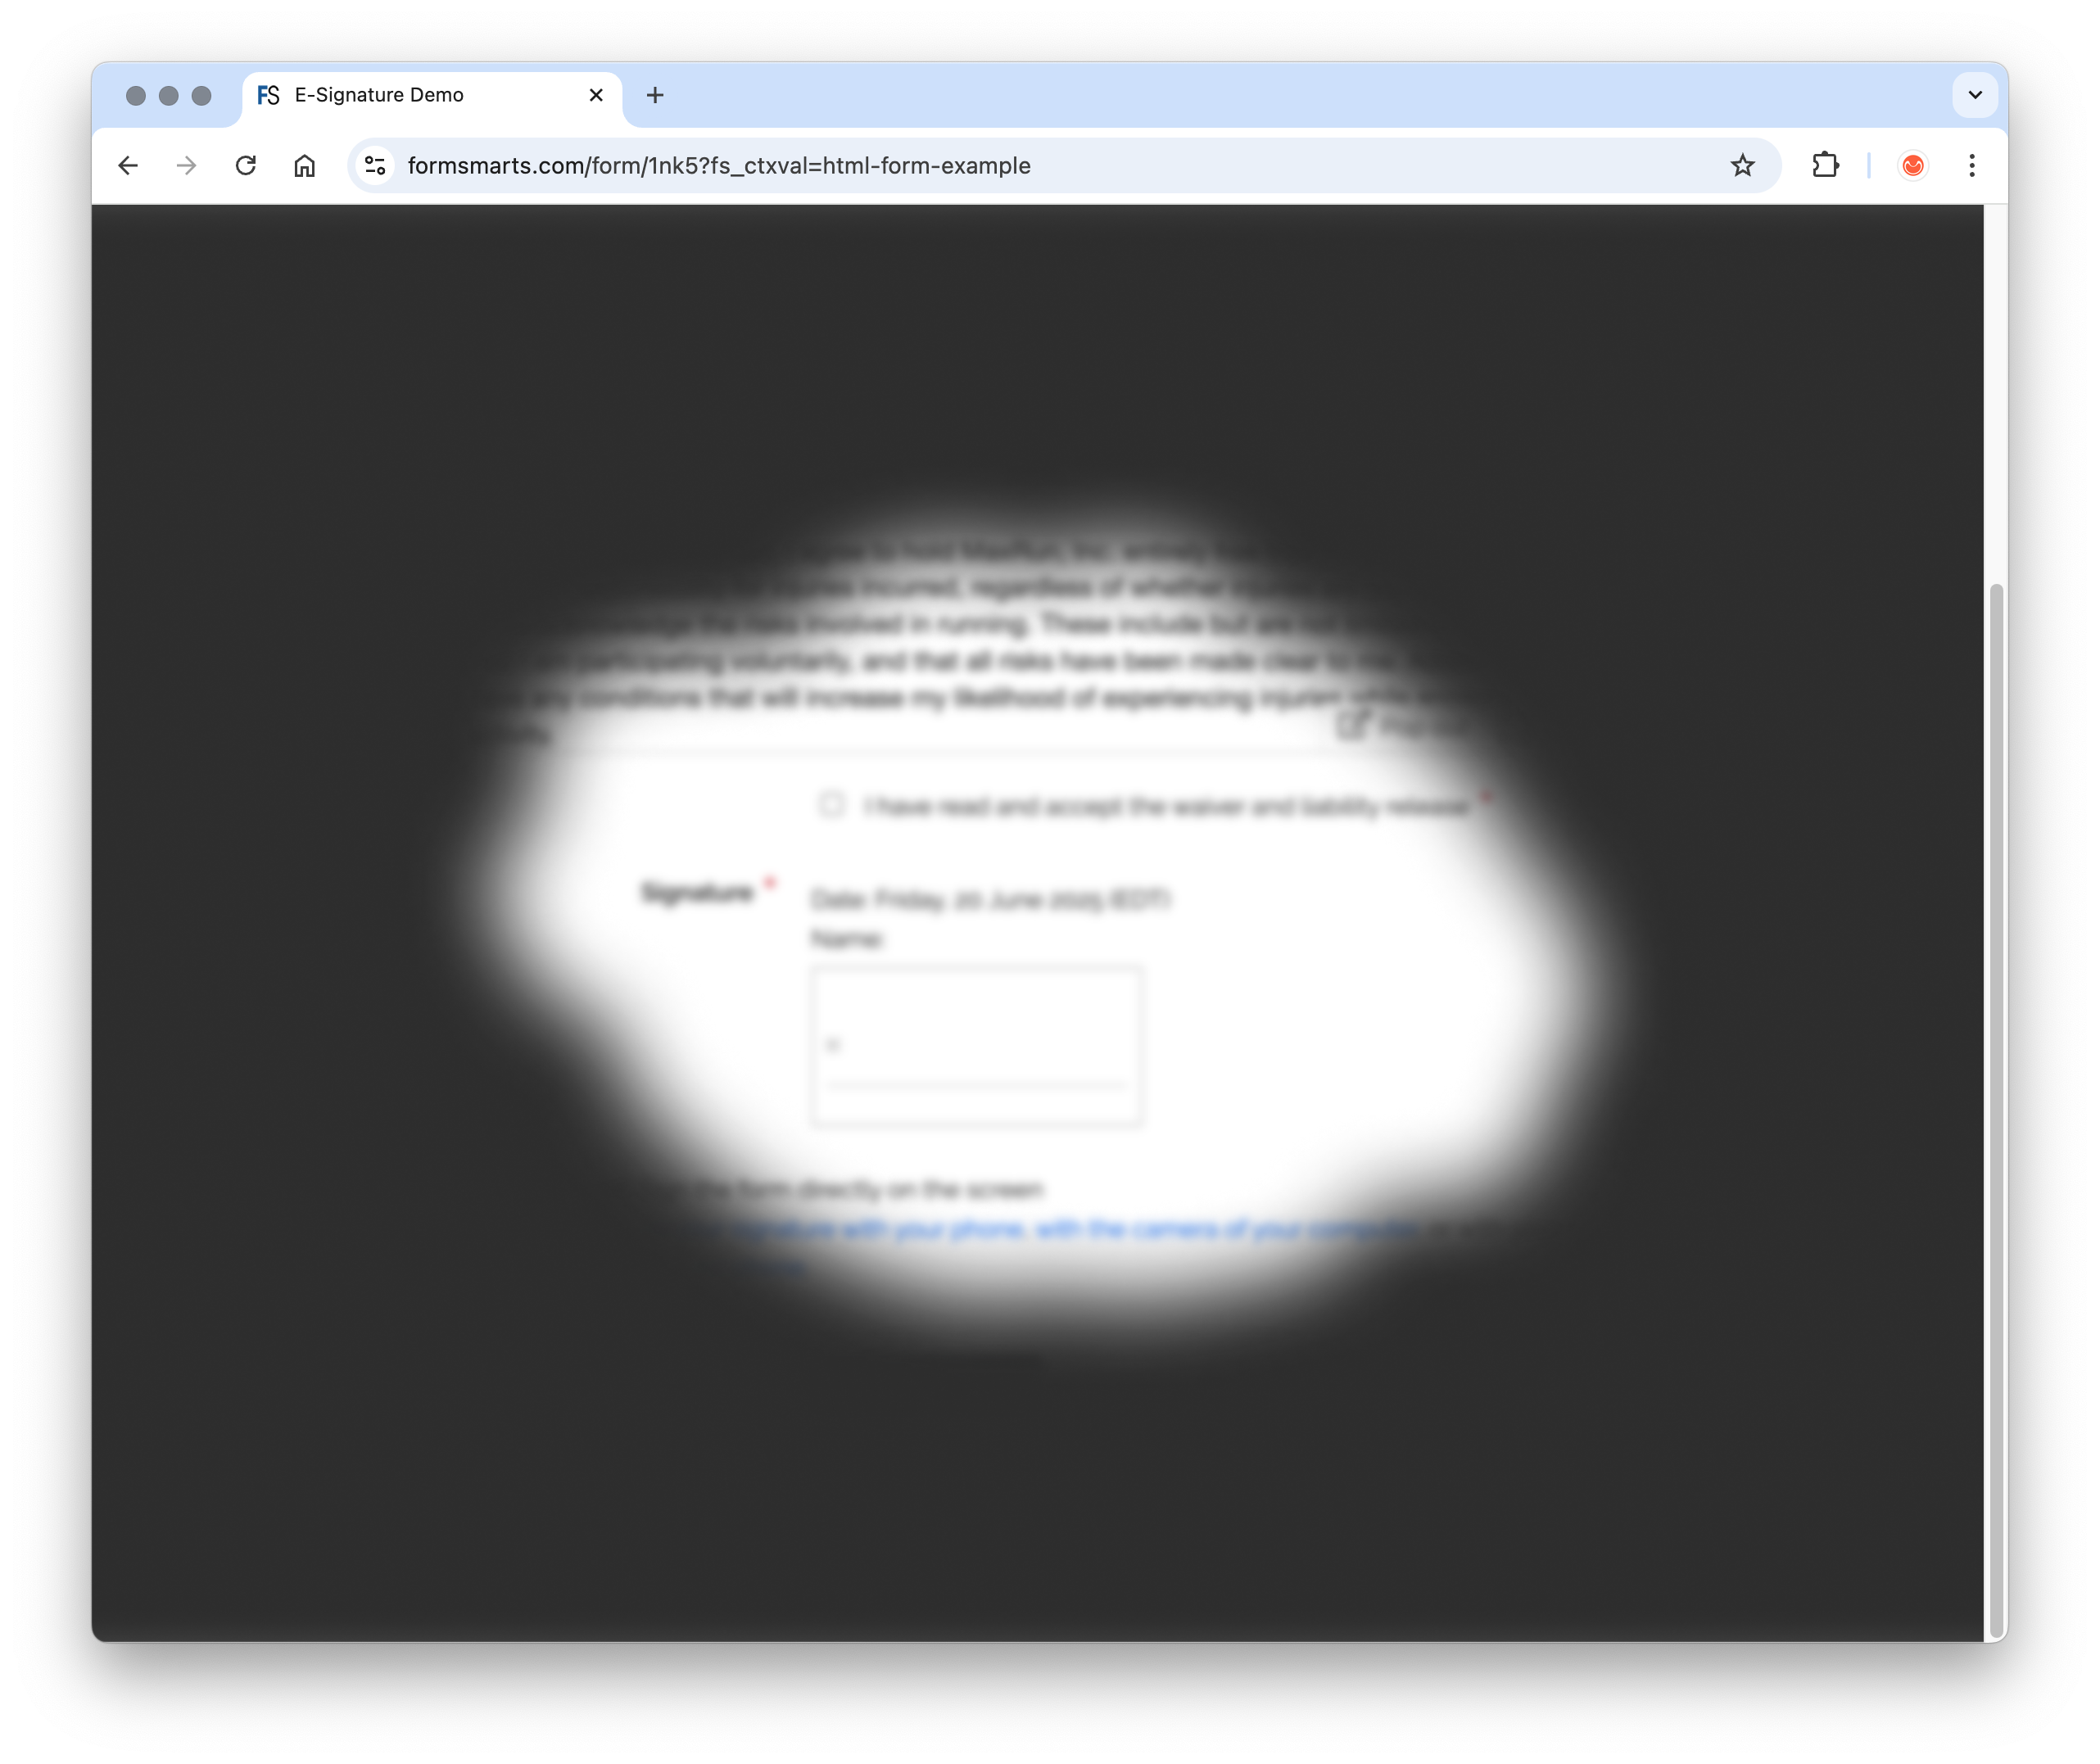
\includegraphics[width=115pt]{imgs/glaucoma-filter.png}
    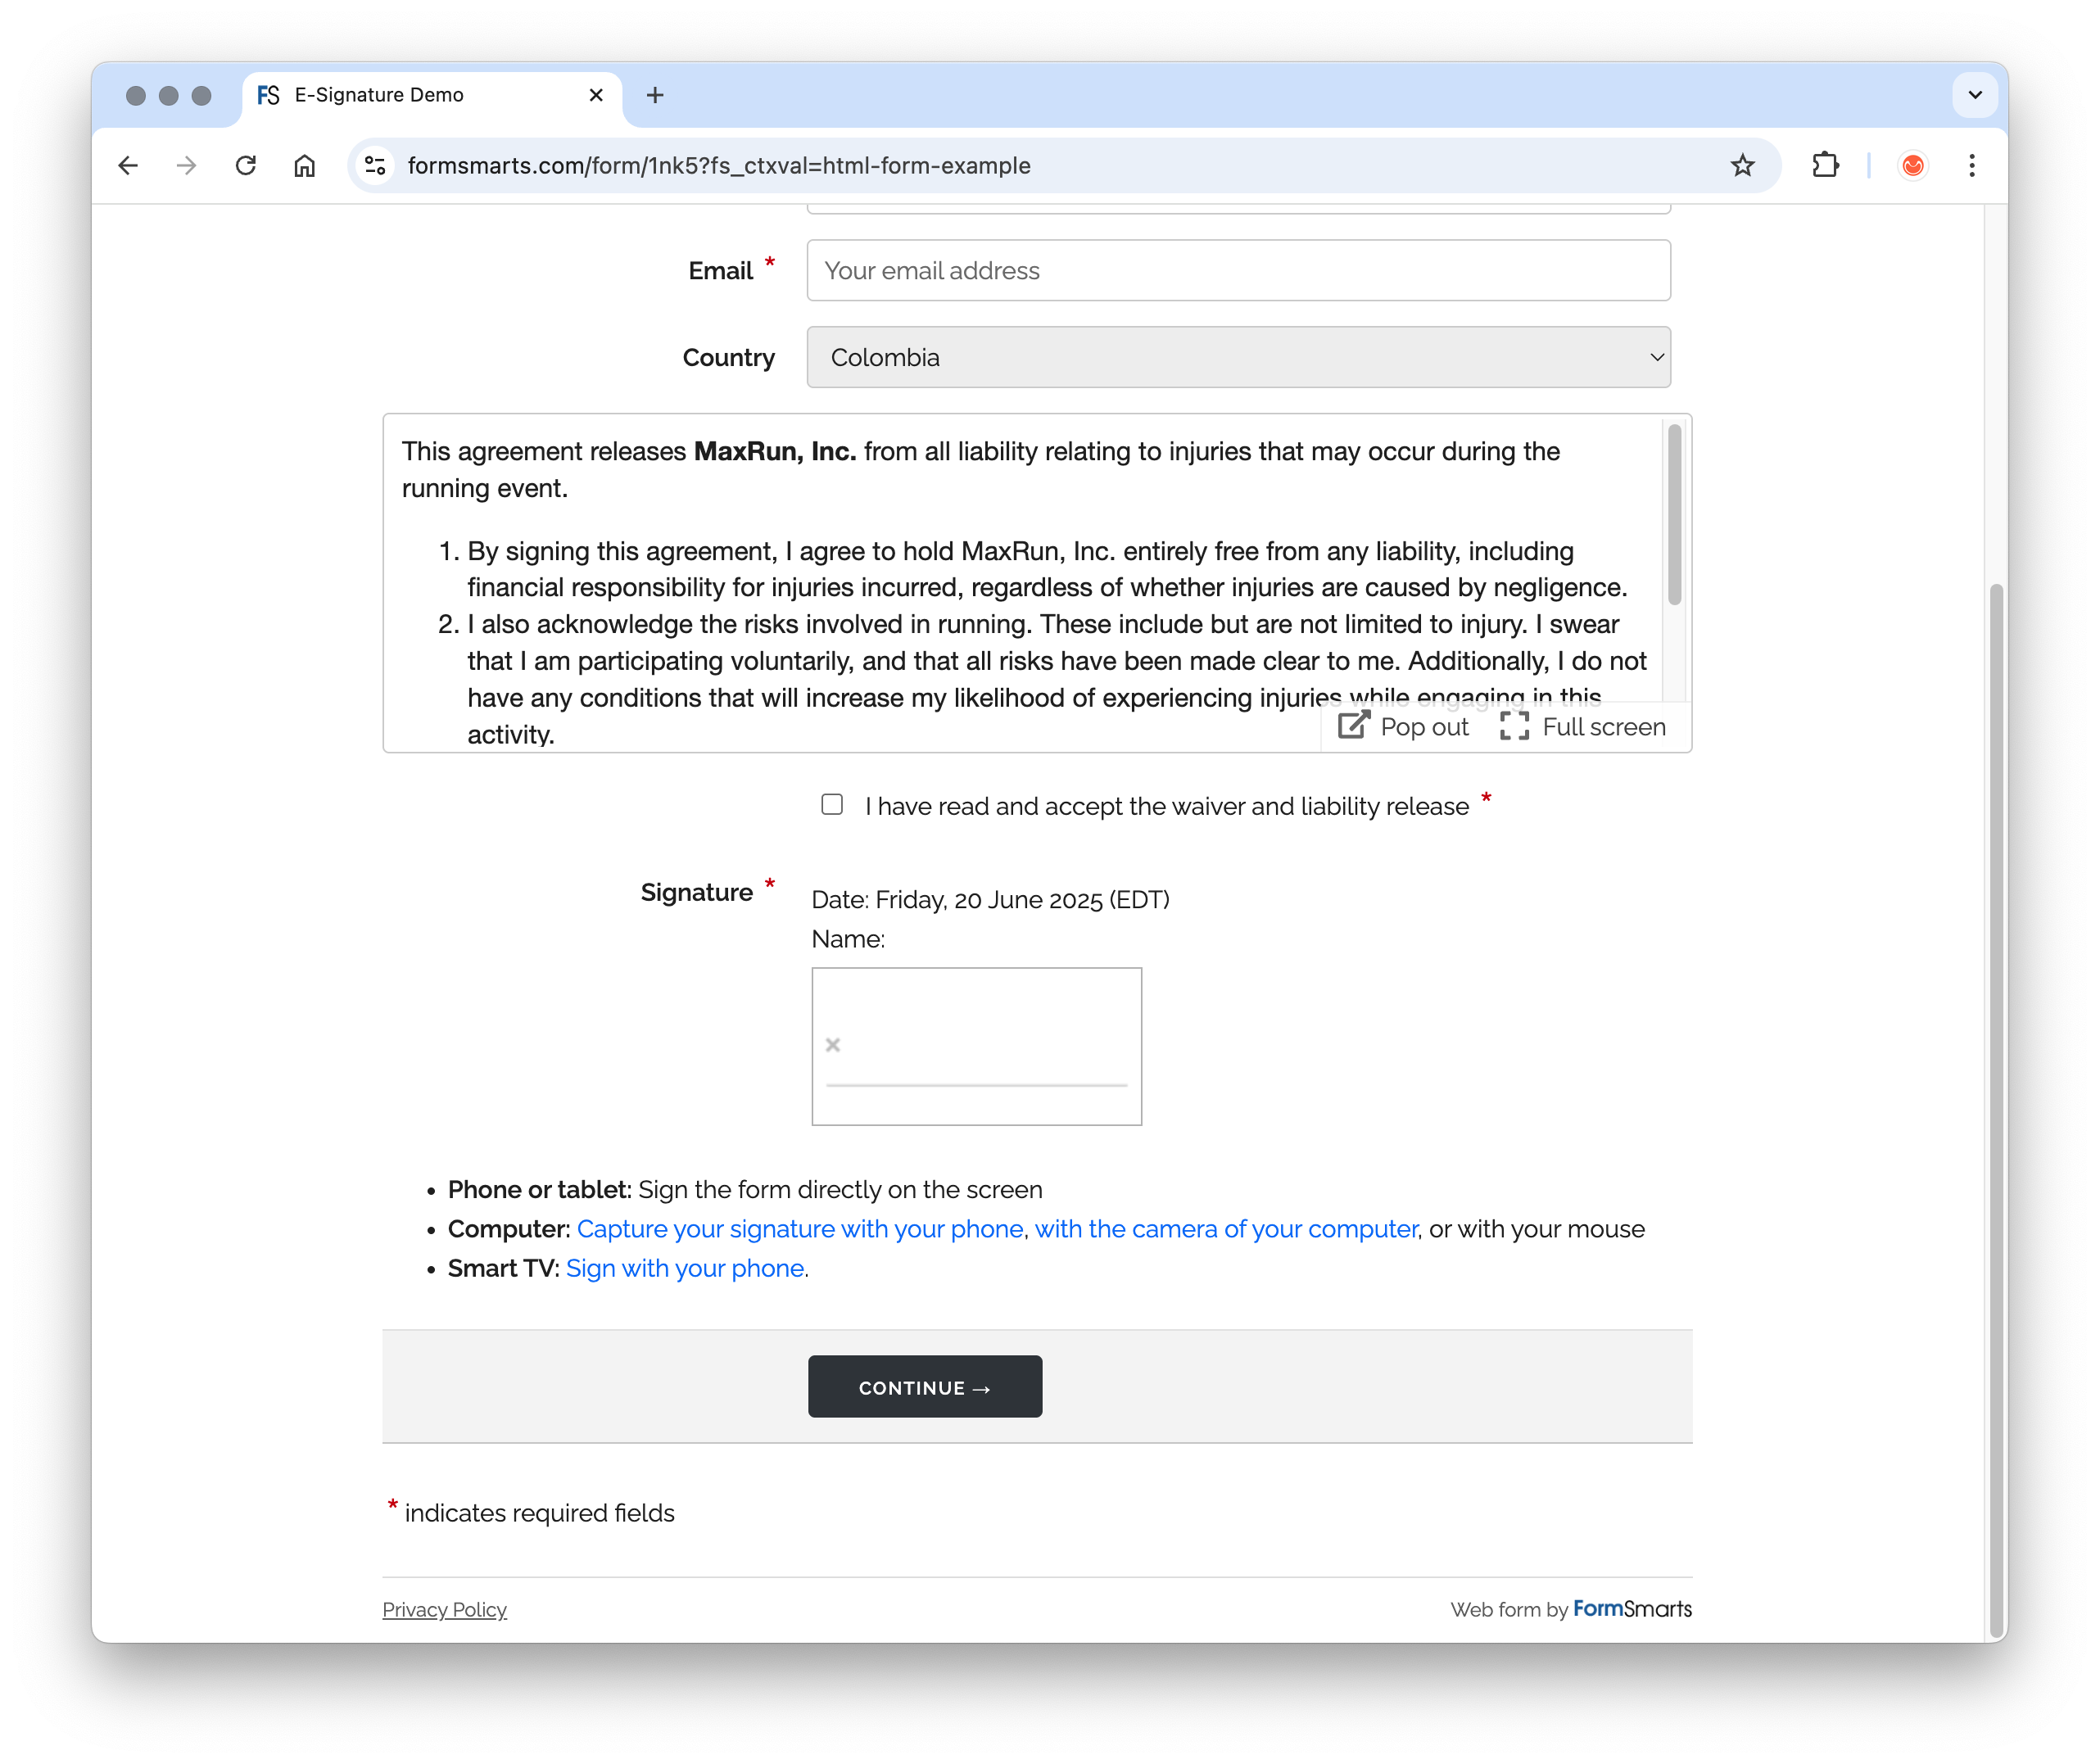
\includegraphics[width=115pt]{imgs/no-glaucoma-filter.png}
    \caption{Left: Glaucoma filter applied to an example form requiring a signature. The "Submit" button is no longer visible, making it difficult to locate. Right: Original version.}
    \label{fig:glaucoma-filters}
\end{figure}

\begin{figure}
    \centering
    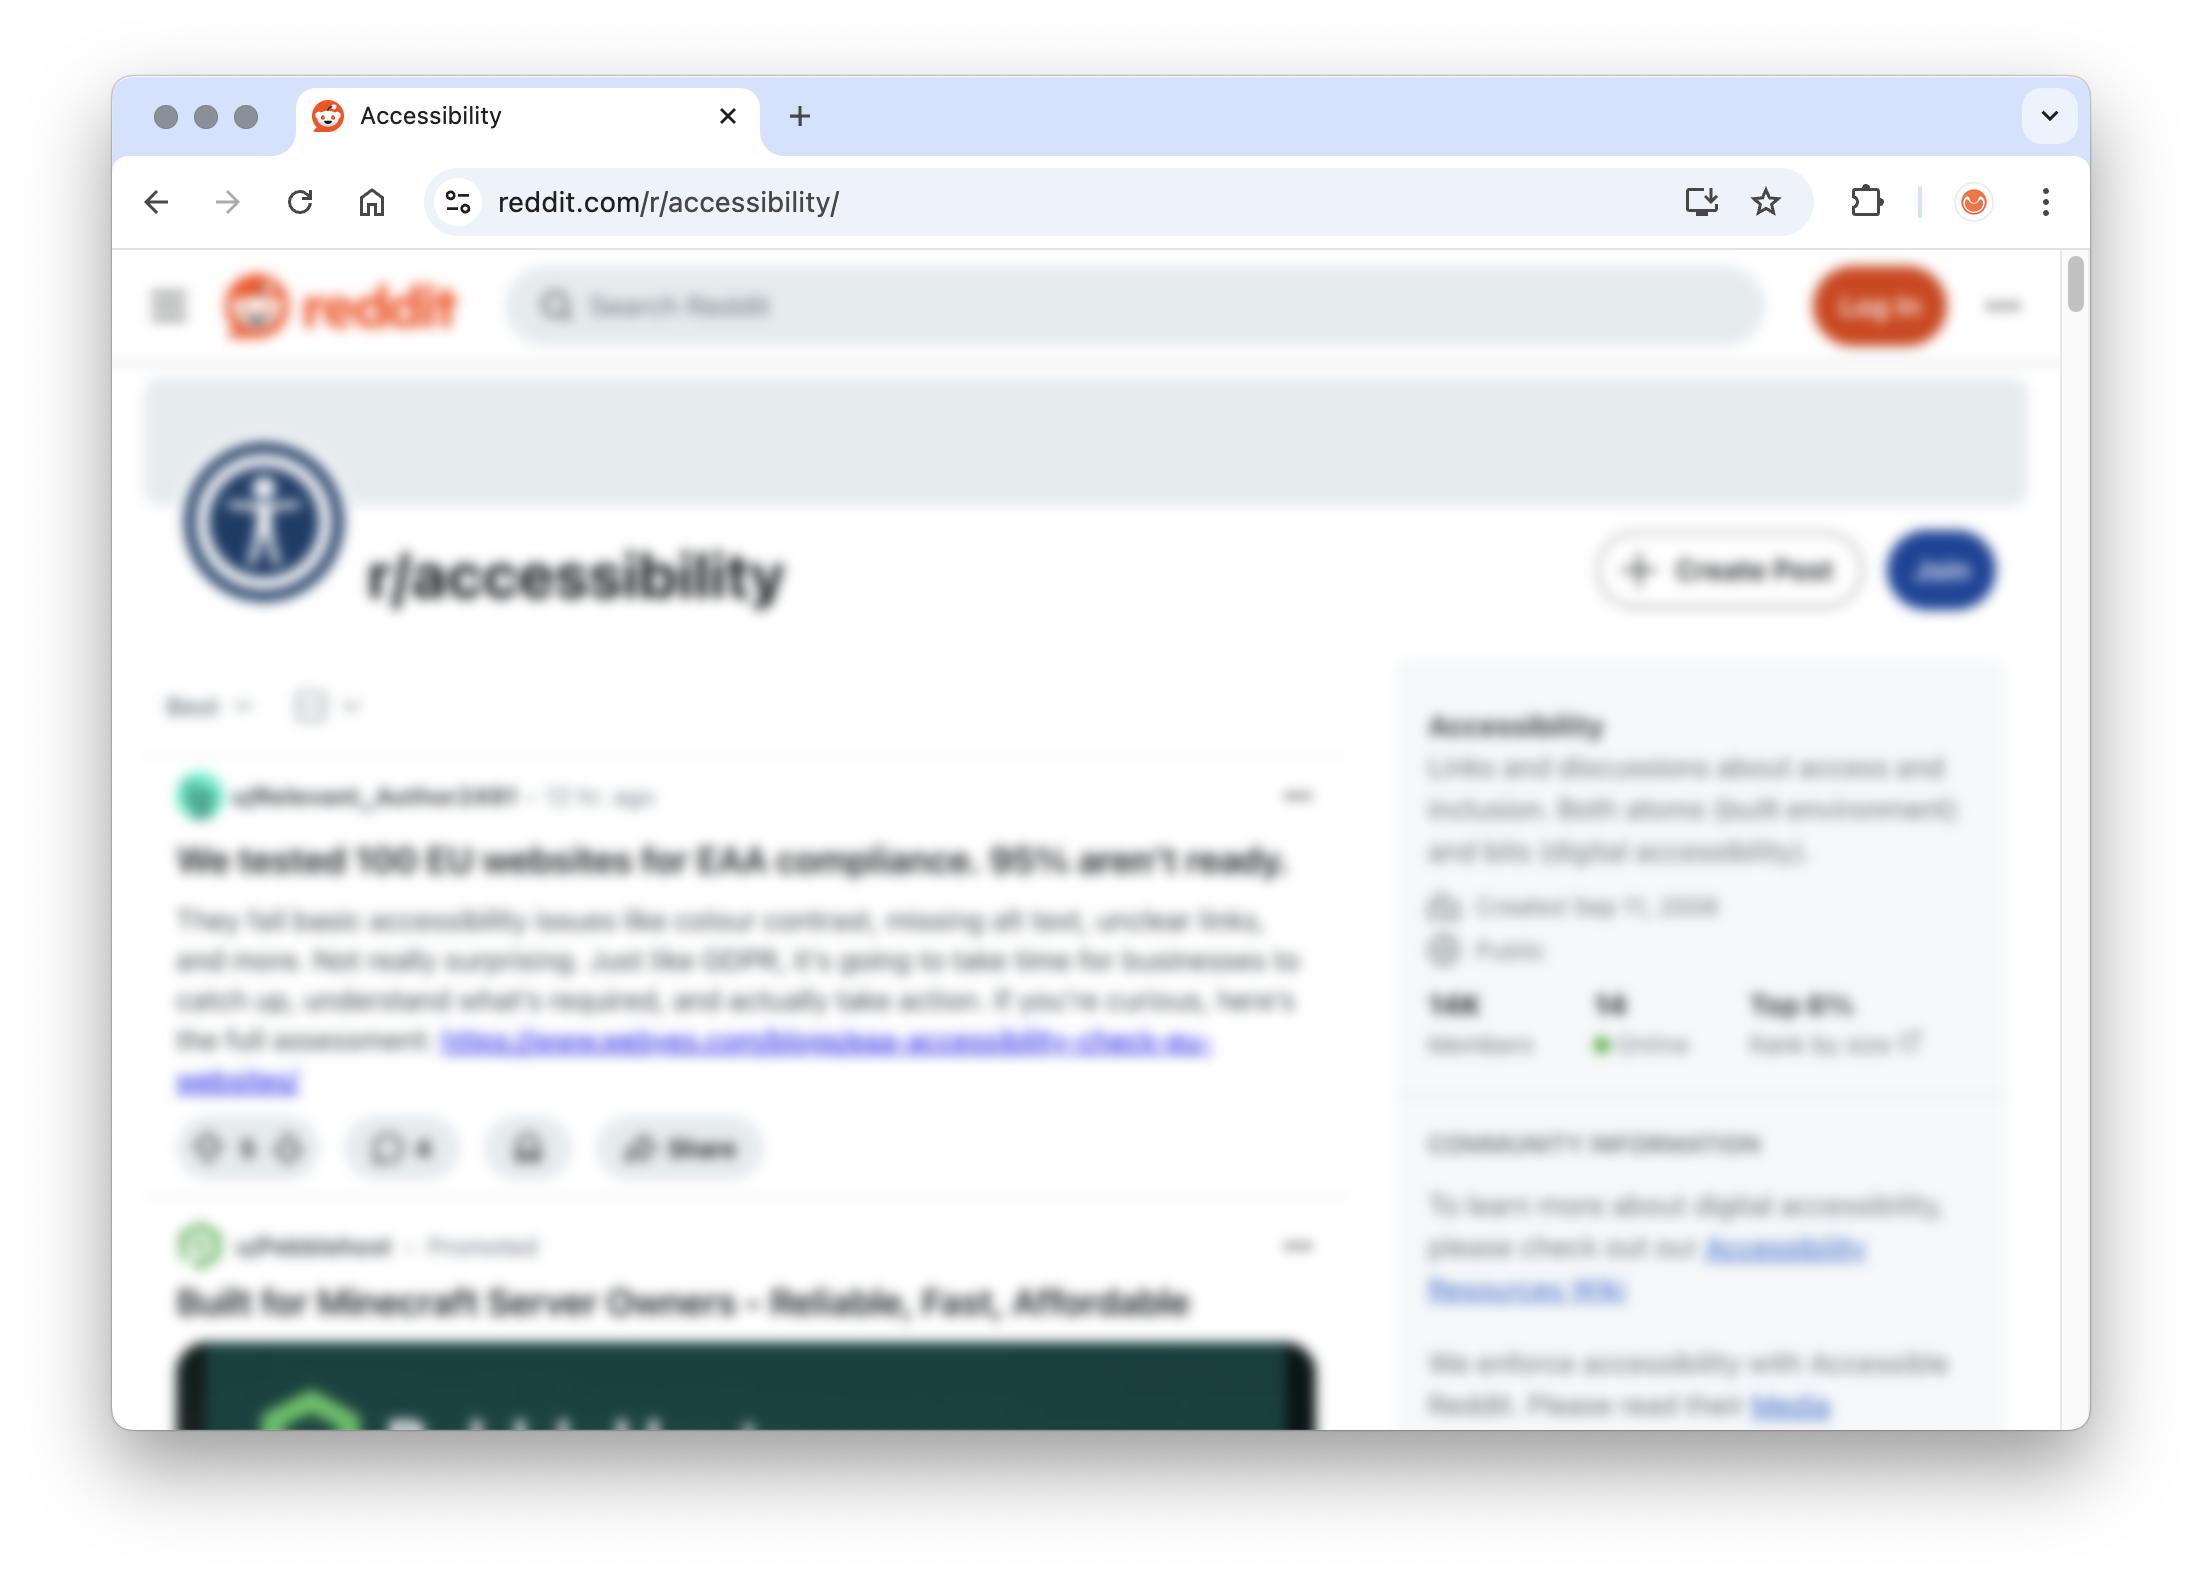
\includegraphics[width=115pt]{imgs/myopia-filter.png}
    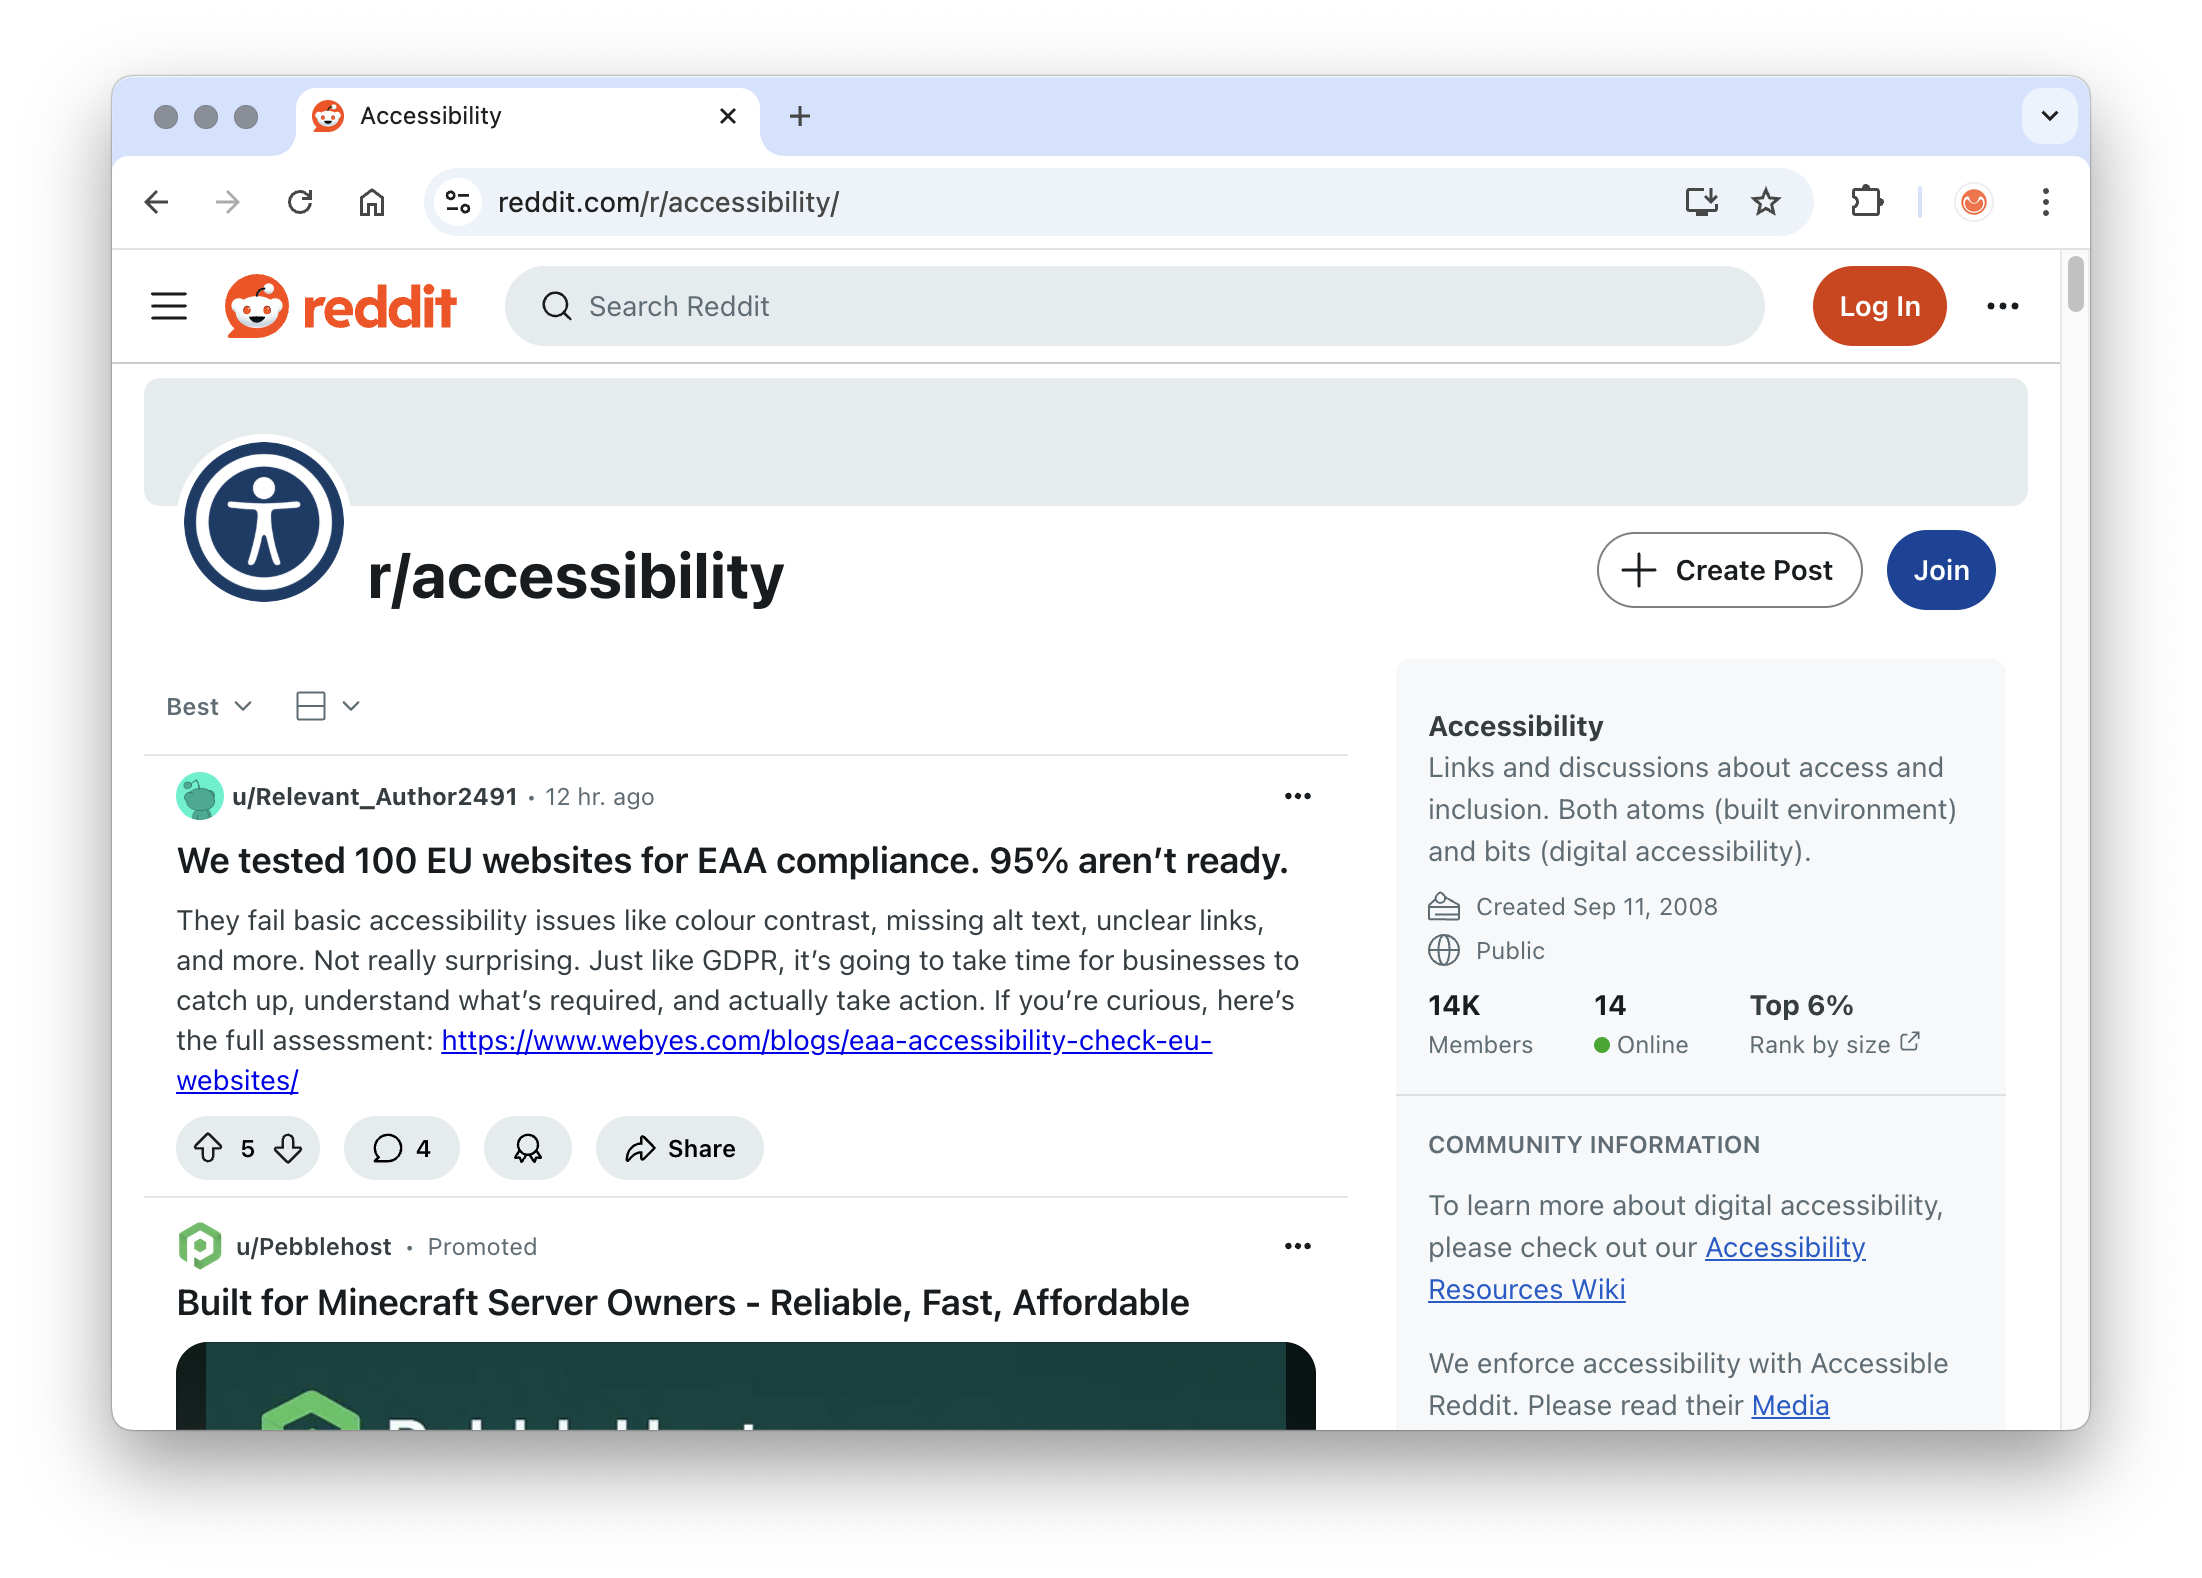
\includegraphics[width=115pt]{imgs/no-myopia-filter.png}
    \caption{Left: Myopia filter (-3 diopters) applied to a social media webpage, reducing clarity and edge sharpness. Right: Original version.}
    \label{fig:myopia-filters}
\end{figure}

These simulations (see figures. \ref{fig:glaucoma-filters} and \ref{fig:myopia-filters}) were implemented using the Visual Impairments Simulator Chrome extension \cite{visual_impairments_simulator}. While such tools provide a useful approximation of typical visual conditions, they are inherently limited: visual disabilities are highly individualized, and no filter can perfectly replicate the subjective visual experience of every user.

Future work should involve collaboration with ophthalmologists, vision science and other experts to improve the realism and clinical accuracy of these filters. Their insight can guide the calibration of filter parameters and help us design simulations that more closely resemble the lived experiences of users with specific visual conditions.

\subsection{Assistive output integration}

\begin{figure}
    \centering
    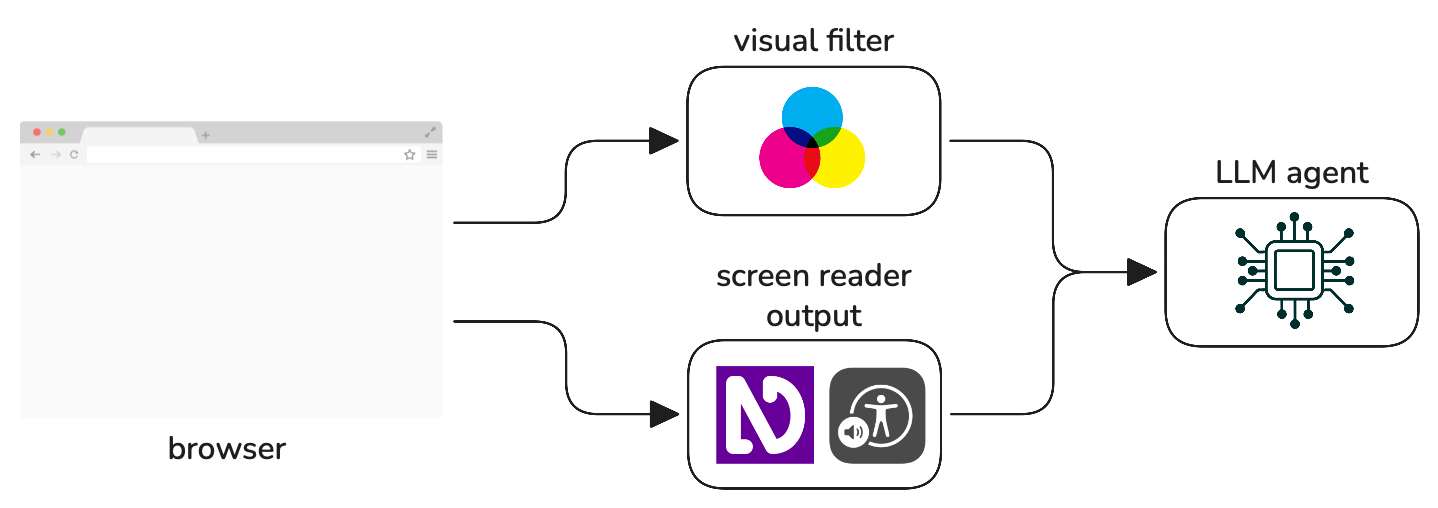
\includegraphics[width=1\linewidth]{imgs/flow.png}
\caption{Proposed pipeline for the agent feeding inputs}
\label{fig:pipeline}
\end{figure}


The agent must capture what an assistive technology user would hear and do. For screen reader output, we can integrate a driver API, such as Guidepup that programmatically controls VoiceOver (macOS) or NVDA (Windows). This driver issues the same keyboard commands a user would and exposes the spoken utterances\cite{guidepup2025}. The agent framework would invoke this API at each step and record the resulting string of text (including element role, name, state) as sensory input.

For keyboard-only navigation logs, the agent can log focus events. As the agent presses Tab, arrow keys, Enter, etc., a browser automation framework, such as Playwright, Selenium or Kraken, can attach listeners to record each focus transition and action. This yields a sequence of elements visited in order\cite{ravelo2023kraken}. These logs serve two purposes: they ensure the agent only uses keyboard input, and they provide a trace of the navigation path for later analysis and execution. For instance, the log can reveal if an item was skipped or if the focus order was non-standard. Together, these multimodal streams visual focus shifts and spoken labels populate the agent's perception at each timestep. This proposed pipeline can be visualized in figure \ref{fig:pipeline}.

The agent may optionally inspect the page for accessibility metadata, thereby having the ability to cross-check perception. This means reading the ARIA attributes for the current focused element. For instance, when an element is in focus, the agent can query its \verb|aria-label|, via de Accessibility Object Model or other APIs. %este es el otro arbol dom de solo accesibilidad
This is then compared to the other information (visual, audio). If the visible text of a button says “Search” but its ARIA label is “Submit,” that mismatch is noteworthy. Likewise, this is helpful for alt text. If the alt text of an image is \verb|alt= 'Company Logo'| but the screen reader says "Image", it indicates a missing accessible name. This is useful for verifying consistency, which is one of the guidelines on \ac{WCAG} and IBM's\cite{ibm2025accessibility}.


\subsection{Decision and Action Module}

Our approach consists of prompting the agent with a basic user goal, such as “given this screenshot and screen reader transcript, where is the 'Submit' button?” The agent will then attempt to complete the task, using the screen reader and seeing through the visual impairment filter applied to the interface.

For example, one scenario may involve an \ac{AI} agent attempting to find and click a "Submit" button after filling out a form. With a glaucoma filter applied (see Fig. \ref{fig:glaucoma-filters}), the button may become difficult to distinguish due to peripheral blur or low contrast.


\subsection{Workflow Definition}

Each testing task needs to be defined in advance. This can be done either with a script or using natural language to define a goal. Then, the agent will execute said task in a closed loop that has a completion or failure condition. The loop can be structured in this way

\begin{enumerate}
    \item Perception: Capture the current \ac{UI} state. This includes a screenshot of the page and the latest screen-reader output. Optionally also collect DOM/ARIA info for elements in focus. 
    \item Decision: Use the agent's strategy to choose the next action. An LLM-based agent might generate a plan (e.g. “click the Login button”) from the task description, and then a rule-based agent would follow a predetermined script (e.g. “press Tab until username field is focused, then type”).
    \item Action: Execute the chosen step.
    \item Measure: Record relevant outputs. Log the agent's action, the resulting new screen-reader output, and any state changes. Check if the task goal is reached. If not, loop back with the new perception.
\end{enumerate}



\subsection{Metrics and Analysis}

After execution is complete, some of the metrics we propose that the system displays are both classic usability and accessibility-specific. These include the agent's task success rate, efficiency (measured by completion time or number of actions), and the frequency of interaction errors such as missed clicks or incorrect actions that require backtracking. We also include the consistency between screen reader output and the visible \ac{UI}, flagging any mismatches between spoken labels and on-screen text or roles. Visual robustness can also be examined by analyzing the webpage before the filter, discovering layout faults like overlapping or off-screen elements, among others. Heuristic checks are performed during testing, such as verifying that text scales appropriately in high-contrast or large-text modes and monitoring for navigation loops. Throughout the process, we aggregate logs of the agent's actions and screen reader output for offline analysis, enabling manual review or further explanation by the agent. By comparing these metrics across different simulated conditions, we can quantify the impact of visual impairments on usability and identify both layout and semantic accessibility issues.

% \subsection{Ethical Considerations}

% Simulated agents must not be seen as full substitutes for real users with disabilities. They are procies, and never replacements for real user studies. Their effectiveness depends on how accurately they model user behavior, and poor design could lead to misrepresentations of user needs. Eventual human validation is also necessary, to ensure no mismodeling and to take into account privacy considerations.


\section{Evaluation}

To investigate the feasibility and effectiveness of using autonomous AI agents for accessibility evaluation, we pose several research questions. First, we ask whether autonomous AI agents can realistically emulate the interaction patterns of users with vision-related impairments when navigating web interfaces. This includes examining which visual filters or perceptual constraints most effectively represent different types of visual impairments in a simulated context, and what design principles are necessary for agents to approximate impaired visual perception through perception-based (rather than code-aware) interaction.

We also explore whether these agents can surface accessibility problems that static tools overlook, such as poor contrast visibility, confusing focus order, or dynamic content that is not screen-reader friendly. Another important question is whether agent-based testing, when combined with simulated impairments, can produce accessibility assessments that are reliable and generalizable. We are interested in the extent to which LLM-powered agents or learning-based systems can internalize accessibility heuristics through observation of human interaction data, rather than relying solely on static rule sets.

% Ethical considerations are central to this research. We examine the risks that arise when relying on simulated agents as stand-ins for real users with disabilities, particularly in terms of misrepresentation or oversimplification. We seek to ensure that agent-based evaluation tools meaningfully contribute to more inclusive web design, rather than substituting for real user feedback, and that agents simulating disabilities preserve the autonomy and dignity of real users, rather than acting as complete surrogates.

Finally, we investigate how combining simulated visual impairment filters with screen reader output affects the agent's ability to detect accessibility issues, and whether multi-modal input can uncover problems, such as missing alt text, that would not surface if using only visual filtering.

Our evaluation plan involves initial experiments using a set of benchmark pages, such as public websites with known accessibility issues. We will define tasks like form submission and navigation, and compare agent results under different filters and input modes. In future work, we may include qualitative validation with accessibility experts or small user studies to further assess the reliability and generalizability of agent-based accessibility evaluations.

% !TEX root = main.tex

\section{Conclusion \& Future Work}

This paper proposes a new direction for accessibility evaluation: the use of autonomous, multi-modal \ac{AI} agents that simulate visual impairments and interact with web content through perception, not code. By combining visual filters, screen reader output, and task-based prompting, this approach aims to approximate the experiences of users with diverse visual disabilities and to surface accessibility issues that may be missed by static tools.

The potential of this method lies in its ability to reveal failures that only emerge under perceptual constraints, and to provide richer, multi-modal insights into web accessibility. At the same time, we recognize the ethical and methodological challenges of using simulated agents as proxies for real users, and stress the importance of human validation.

As next steps, we plan to design and implement a prototype system that integrates visual impairment simulation, screen reader emulation, and agent-based control. We will define representative tasks and benchmark scenarios to explore how different impairments and input modes affect accessibility outcomes. Future work will also involve comparing this approach with existing static tools, and seeking feedback from accessibility experts and users. Ultimately, we hope this research will lay the groundwork for more dynamic, user-centered accessibility evaluation methods and inspire further investigation in this area.


% \section*{Acknowledgment} 


\balance
\bibliographystyle{IEEEtran}
\bibliography{local,bib/testing,bib/tools}

\end{document}
